\chapter{Overview}
The content of this chapter provides definitions and explanations of terms and methods used in the following chapters with intention to aid in understanding the topic discussed in this thesis.

\section{Anthropometry}
Our goal in this thesis is to estimate human body measurements. These are important for certain tasks as clothing sewing, virtual environment calibration, creating realistic avatars and more. For these task we need a set of measurements which will guide us. Measurement locations vary by the use, and thus there is no universal guide. Professionals should be familiar with the measurements required in their field of application, but the subjects themselves are usually not as informed. This can then result in incorrect measurement. Using a trained neural network model can prevent that. Another advantage of using a neural network is the speed of measurements. Compared to manual measurement, our neural network based approach can estimate multiple measurements at once, whereas while using the manual approach we only get one measurement at a time. This makes our approach easier to use than 

The human body can be measured using different methods. These are usually dependent on input data, and thus not every method can be used in every situation.  

\subsection{Manual measurement}
This is the traditional method of using tape or any similar measuring device to obtain measurements. The approach usually requires one extra person who performs the measurement on the subject. Due to measurements that must be taken at specific locations to provide correct information, a person without help is more prone to obtaining incorrect measurements.


\subsection{Virtual measuring on 3D model}
Another method used to obtain measurements is the use of scanning technology. One of the approaches uses devices such as photogrammetry scanners to create realistic meshes of the scanned subject. The data can then be registered to the mesh topology of SMPL \cite{smpl}. We can then use the resulting mesh to calculate the required measurements. This is also the case for \cite{BodyM}, which uses these measurements as ground-truth data. 
A different approach uses 3D scanning devices. These are more expensive than the equipment required for photogrammetry, but they can provide precise models. The result of a scan using a 3D scanner is a point cloud or a set of data points that represent the shape and size of the subject~\cite{3dScan}. This can be used directly as input for further processing.
\subsubsection{Photogrammetry scanner}
Photogrammetry scanners utilise photographs from different angles and positions to calculate and create a mesh. The device to take photos does not need any extra functionality to produce images that are processable in the final model. However, photogrammetry scanners are being developed to provide ease of use and quality over common cameras. Scanners can be joined into a multi-camera system. This allows capturing photos from multiple angles simultaneously, which provides more accurate data compared to using a single camera  setup.
\subsubsection{3D scanner}
Another type of scanner is the 3D scanner, which employs various techniques to measure the distance from the camera to the subject. Commonly used methods include structured light and laser-based scanning. Both techniques use light to determine the location of points on the subject. Laser-based scanners project lines onto the subject and record the reflections, while structured light scanners project a grid pattern. By analyzing the distortions in the reflected light, these devices can accurately measure distances and create detailed 3D models.

\section{SMPL}
SMPL, an acronym for Skinned Multi-Person Linear model \cite{smpl}, is a versatile tool for generating animated human bodies with diverse body shapes and specific poses. One of its notable features is its ability to simulate natural soft-tissue deformation, resulting in lifelike movements. This is achieved through the integration of blend shapes and joints.

Blend shapes in SMPL are defined as a vector of concatenated vertex offsets. Each blend shape is a predefined deformation of the mesh, which, when combined, can represent complex changes in body shape and pose. Essentially, these are sets of vertices that, when adjusted, morph the mesh to match various body forms and postures. By linearly blending these shapes, SMPL can produce a wide range of realistic human body shapes. By using blend shapes, the model can adapt to subtle changes in body shape caused by muscle movement, fat distribution, and individual anatomy.

The SMPL model incorporates a skeletal structure composed of joints that create a hierarchy creating a skeleton. This skeleton defines the kinematic chain used for pose transformations. Each joint is associated with a specific part of the body, and the movement of these joints dictates the overall pose of the model. The character's skeletal structure is rigged to allow for flexible posing while following anatomical correctness.


\section{Neural Networks}
A neural network is a computational model inspired by the structure and function of the human brain. It consists of interconnected nodes, called neurons, that work together to process information. Each neuron receives input variables, processes them, and passes the results to other neurons. These connections have associated weights that determine the influence of each input on the neuron's output.

Neurons are organized into layers: input layers, hidden layers, and output layers. The input layer receives the initial data, the hidden layers perform intermediate computations, and the output layer produces the final result. The hidden layers are crucial for transforming the input data into the desired output by performing complex operations.

Training a neural network is based on adjusting the weights of the connections. This process, called learning, typically involves comparing the network's output to the correct values (ground truth) and trying to minimize the difference, often through a method known as backpropagation. By iteratively adjusting the weights, the network learns to recognize patterns and relationships within the data that might be difficult for humans to find.

This ability to learn and generalize from data enables neural networks to solve a wide range of problems, from image recognition to natural language processing.

\subsection{Hyperparameter}
A hyperparameter is a parameter that is not learned but chosen by the developer.  These parameters do not change over time. These can be - the choice of optimizer, learning rate,  number of layers, filter size and more.\\\\
\subsection{Loss functions}
The training process is guided by the loss function \cite{loss}. They show how good or how bad the network is at predicting the output. The results then serve as a guide for the learnable parameters. The loss function measures the difference between the predicted and expected outputs. The main goal of the network then becomes to minimise the loss function. One of the commonly used losses for regression task such as this one is the mean squared error (MSE sometimes called L2 loss). This loss function is calculated as an average of the squared difference between the predicted values and the ground truth. To define this function mathematically:
\begin{equation}
	MSE = \frac{1}{n}\sum_{i=1}^{n}(y_i -  \hat{y_i})^2
\end{equation}
In this equation $n$ is used to define number of samples, $y_i$ is the ground truth and $\hat{y_i}$ is the predicted value of the $i^{th}$ sample. Being a convex function, the MSE has a unique global minimum, which helps the optimization process as the optimization methods do not get stuck in the local minima. While being computationally simple, it is vulnerable to outliers. The issue is created by the square nature of this function. In the case of an existing outlier, the function gets heavily influenced and may not perform as well.
\\
\subsection{Performance metrics}
After the network is trained on the training data, it has to face new, unseen data. This ability is then measured using performance metrics. They are mainly used after the network has been trained. Performance metrics are also used to compare different networks. We can use some loss functions for performance metrics. In this thesis, we will use mean absolute error (MAE or L1 loss). The principle is similar to MSE, but instead of squaring the difference, we will use the absolute value to always have an error larger than 0, meaning 0 will be a perfect fit. The mathematical definition of the MAE is as follows:
\begin{equation}
	MAE = \frac{1}{n}\sum_{i=1}^{n}|y_i -  \hat{y_i}|,
\end{equation}
in which $n$ is used to define number of samples, $y_i$ is the ground truth and $\hat{y_i}$ the predicted value of the $i^{th}$ sample.

\subsection{Overfitting}
A significant challenge when using neural networks is the risk of overfitting. Overfitting occurs when a complex network is trained on an insufficient amount of data. While the sophisticated architecture of a neural network enables it to capture intricate relationships within the data, a lack of sufficient training data can lead the network to memorize the exact values of the training examples rather than learning the underlying patterns. As a result, the network performs exceptionally well on the training data, exhibiting minimal training loss, but fails to generalize to new, unseen data, resulting in poor performance metrics and larger errors during testing.
\\\\

\subsection{Layers}
Neural networks are composed of layers, each serving a specific purpose in the process of transforming input data into a desired output.  The layers used in our BoMN model are:

\paragraph{Convolution layer}
Most popularly used with convolutional neural networks\\\cite{convolutional} this layer plays an important role in the network's functionality. It is based on working with matrices called kernels.  The values in the kernel are learnable, which means they are adjusted over the training process to enhance performance. In this thesis, we will be using these hyperparameters:
\begin{itemize}
	\item \textbf{Depth} determines the dimension of the output volume (activation maps). Influences pattern recognition as well as the number of neurons.
	\item \textbf{Size} determines dimensions of kernel.
	\item \textbf{Activation function}
\end{itemize}
The algorithm consists of a sliding kernel along the input. At every position, it calculates the sum of the element-wise multiplication of corresponding pixels in the input and kernel. The result is then inserted into the output. This process is then repeated over the whole input multiple times (depending upon the number of kernels) %CHECK THIS WHOLE PART PLEASE 
The result of this operation captures local patterns while preserving positional relationships.


\paragraph{Max Pooling layer}
Max pooling is an operation of non-linear down-sampling. This means that the output image of this layer is usually smaller than the input. This helps to reduce parameters for the next convolutional layer, providing faster training.  This layer is defined by two hyperparameters:

\begin{itemize}
	\item \textbf{Filter size} determines the dimensions. In the case of the filter reaching out of the array, only valid values are taken into consideration.
	\item \textbf{Stride} determines how many columns will the filter move.
\end{itemize}

The higher these hyperparameters' values are the smaller will the output be.\\
%CHECK IF FIELD IS THE CORRECT TERM
This layer iterates over the input field and looks at the subfield with size of filter size. In this subfield, it finds the largest number and writes only the largest number into the output field. After this, the filter moves by stride columns left until all columns are checked. In that case, the filter moves back to the first column of the input field and then moves down by the stride (refer to \ref{maxPooling} as an example).\\ This process is repeated until the whole input field is iterated.

\begin{figure}
	\centering{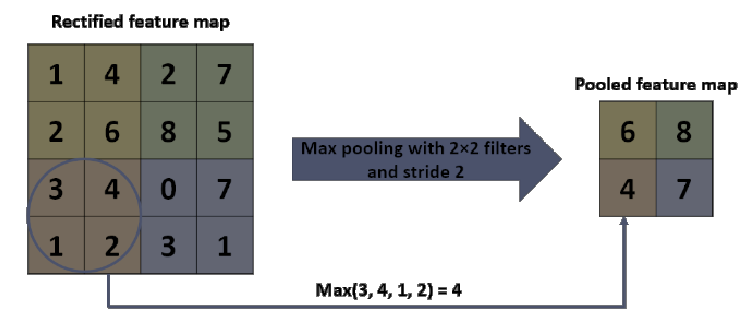
\includegraphics[scale=0.4]{images/MaxPoolingExample}}
	\caption[Max Pooling Example]{Max Pooling Example \cite{pooling}}
	\label{maxPooling}
\end{figure}

\paragraph{Flatten layer}
The flatten layer serves as a bridge between convolutional or pooling layers and dense (fully connected) layers. Convolutional layers and pooling layers often output multi-dimensional tensors, which are unsuitable for direct input into dense layers. The flatten layer transforms these multi-dimensional tensors into a one-dimensional vector, preserving the spatial information. It reduces the dimensions of the input, creating a vector while maintaining the relationship between the data points.
\paragraph{Dense layer}
Dense layers, also known as fully connected layers, are fundamental components of neural networks. In these layers, each neuron is connected to every neuron in the previous layer, enabling feature learning and pattern recognition. Each neuron in a dense layer performs a linear transformation on the input data, followed by the application of an activation function. This process allows the network to learn and combine features from the previous layers, helping the network to understand complex relationships and interactions between them. Dense layers often produce the output, whether it’s class probabilities in classification tasks or continuous values in regression tasks.

The output of a dense layer can be mathematically represented by the equation $y=f(Wx+b)$, where $x$ is the input vector, $W$ is the weight matrix, $b$ is the bias vector, and $f$ is the activation function applied element-wise. This equation describes how the dense layer transforms the input data by applying weights and biases and then passing the result through an activation function, which introduces non-linearity into the model.

Activation functions in dense layers are crucial because they enable the network to learn more complex patterns and relationships. Common activation functions include the Rectified Linear Unit (ReLU)~\cite{relu}, which helps the network handle non-linear relationships while mitigating the vanishing gradient problem,


